\subsection{Abstract}

We write a Fortran program that solves $\ddot{x} - x = 0, x(0)=1, \dot{x}(0)=0$ problem numerically using a finite-difference method. We plot the numerical solution and compare it with the exact solution. We look at absolute errors of numerical solutions and investigate their dependence on the size of the time step. We find that global errors of our numerical method are proportional to the square of the time step for time steps between $0.0005$ and $1$. Using time steps smaller than $0.0005$ result in increase of the errors.

\subsection{The ODE}

We want to use a finite-difference method in order to numerically solve the second order linear homogeneous ordinary differential equation
\begin{equation}
  \ddot{x} + x = 0,
  \label{eq_ode}
\end{equation}
that has initial conditions
\begin{align}
  x(0) &= 1 \label{eq_ode_condition_one} \\
  \dot{x}(0) &= 0. \label{eq_ode_condition_two}
\end{align}



\subsection{Finding exact solution}

We will first find the general solution to \autoref{eq_ode}. The corresponding characteristic equation is:
\[
  \lambda^2 + 1 = 0
\]
with roots:
\[
  \lambda = \pm i.
\]
Therefore, the general solution to \autoref{eq_ode} is
\begin{equation}
  x = A \cos t + B \sin t, \quad A, B \in \mathbb{R}.
  \label{eq_general_solution}
\end{equation}
Next, we use the initial conditions to find the values of constants $A$ and $B$. Using \autoref{eq_ode_condition_one} gives
\begin{align*}
  x(0) &= 1 \\
      &= A \cos 0 + B \sin 0 \\
      &= A.
\end{align*}
Therefore,
\[
  A = 1.
\]
Next, we calculate the derivative of $x$ using \autoref{eq_general_solution}:
\begin{align*}
  \dot{x} &= -\sin t + B \cos t.
\end{align*}
Applying condition from \autoref{eq_ode_condition_two} gives
\begin{align*}
  \dot{x}(0) &= 0 \\
      &= -\sin 0 + B \cos 0 \\
      &= B.
\end{align*}
We have found that
\[
  B = 0.
\]
Finally, we substitute the values of $A$ and $B$ back into \autoref{eq_general_solution} and find the solution we desired:
\[
  \boxed{x = \cos t.}
\]


\subsection{Deriving a recurrence relation}

Next, we want to find a recurrence relation for solving \autoref{eq_ode} numerically. We begin by writing an approximation of the second derivative:
\[
  \ddot{x} \approx \frac{x(t + \Delta t) - 2 x(t) + x(t - \Delta t)}{\Delta t^2}.
\]
Solving for $ x(t + \Delta t)$ gives
\begin{equation}
  x(t + \Delta t) \approx - x(t - \Delta t) + 2 x(t) + \Delta t^2 \ddot{x}
  \label{eq_exact}
\end{equation}
Next, we use approximations
\begin{align*}
  x_{i-1} &\approx x(t - \Delta t) \\
  x_{i} &\approx x(t) \\
  x_{i+1} &\approx x(t + \Delta t), \quad \textrm{for} \ i = 0, 1, \dots , n_t,
\end{align*}
where $n_t$ is the number of time steps.
With the approximations \autoref{eq_exact} becomes
\begin{align*}
  x_{i+1} &= - x_{i-1} + 2 x_{i} + \Delta t^2 \ddot{x_{i}} \\
    &= - x_{i-1} + 2 x_{i} - \Delta t^2 x_{i} \tag{Use \autoref{eq_ode}}\\
    &= - x_{i-1} + x_{i} (2 - \Delta t^2 ).
\end{align*}
Finally, we replace $i$ with $i+1$ in order to make the indexes start from $0$ and not from $-1$ and get the recurrence relation we wanted:
\begin{equation}
  \boxed{ x_{i+2} = - x_{i} + x_{i+1} (2 - \Delta t^2 ), \ i = 0, 1, \dots , n_t }
  \label{eq_reccurence_relation}
\end{equation}

\subsection{Calculating $x_1$}

We have found out recurrence relation but we can't use it yet: we know
\[
  x_0 = 1 \tag{from \autoref{eq_ode_condition_one}},
\]
but we don't know $x_1$. In order to estimate $x_1$, we use a power series expansion around $t=0$:
\[
  x(0 + \Delta t) \approx x(0) + \dot{x}(0) \Delta t + \frac{1}{2} \ddot{x}(0) \Delta t^2.
\]
Next, we substitute $\ddot{x}$ from \autoref{eq_ode}, as well as $x$ and $\dot{x}$ from Equations \ref{eq_ode_condition_one} and \ref{eq_ode_condition_two}:
\[
  x(\Delta t) \approx 1 - \frac{1}{2} \Delta t^2
\]
Finally, we substitute approximation
\[
  x_1 \approx x(\Delta t)
\]
and find the expression for $x_1$ that we wanted
\[
    \boxed{ x_1 = 1 - \frac{1}{2} \Delta t^2. }
\]


\subsection{Calculating full numerical solution}


Next, we write a Fortran program that solves \autoref{eq_ode} numerically. The program is given the size of the time step $\Delta t$, as well as the final value of $t$. The starting value of $t$ is set to be zero by the initial value conditions. The first two values of $x$ are
\begin{align*}
  x_0 &= 1 \\
  x_1 &= 1 - \frac{1}{2} \Delta t^2.
\end{align*}
The remaining values are calculated iteratively using the recurrence relation from \autoref{eq_reccurence_relation}.


Instructions for compiling and running the program are located in the README.md file that comes with the source code.


\subsection{Plotting approximate and exact solutions}

We plot the approximate and exact solutions of \autoref{eq_ode} on \autoref{fig_approx_vs_exact_dt_1} for $\Delta t = 1$. We can see that this time step does not result in good agreement between two solutions. Next, we decrease the time step to $\Delta t = 0.1$, as shown on \autoref{approx_vs_exact_dt_0_1}. Now the approximate solution looks indistinguishable from the exact one on this scale.
\begin{figure}[H]
  \centering
  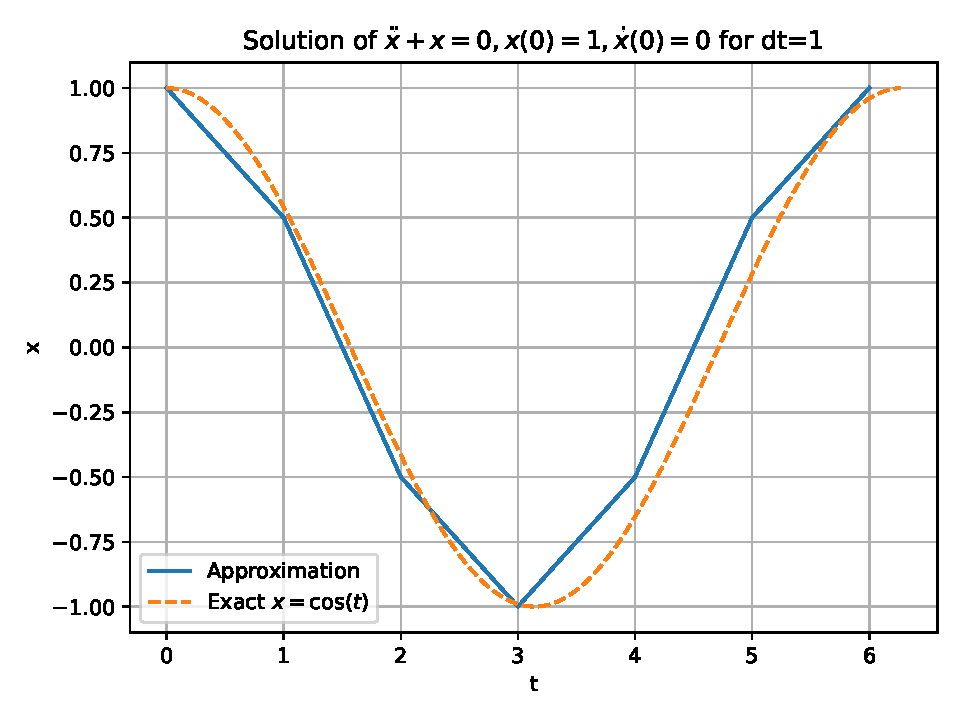
\includegraphics[width=0.8\textwidth]{figures/approx_vs_exact_dt_1.pdf}
  \caption{Approximate and exact solutions of the problem $\ddot{x} - x = 0, x(0)=1, \dot{x}(0)=0$ for $\Delta t = 1$.}
  \label{fig_approx_vs_exact_dt_1}
\end{figure}
\begin{figure}[H]
  \centering
  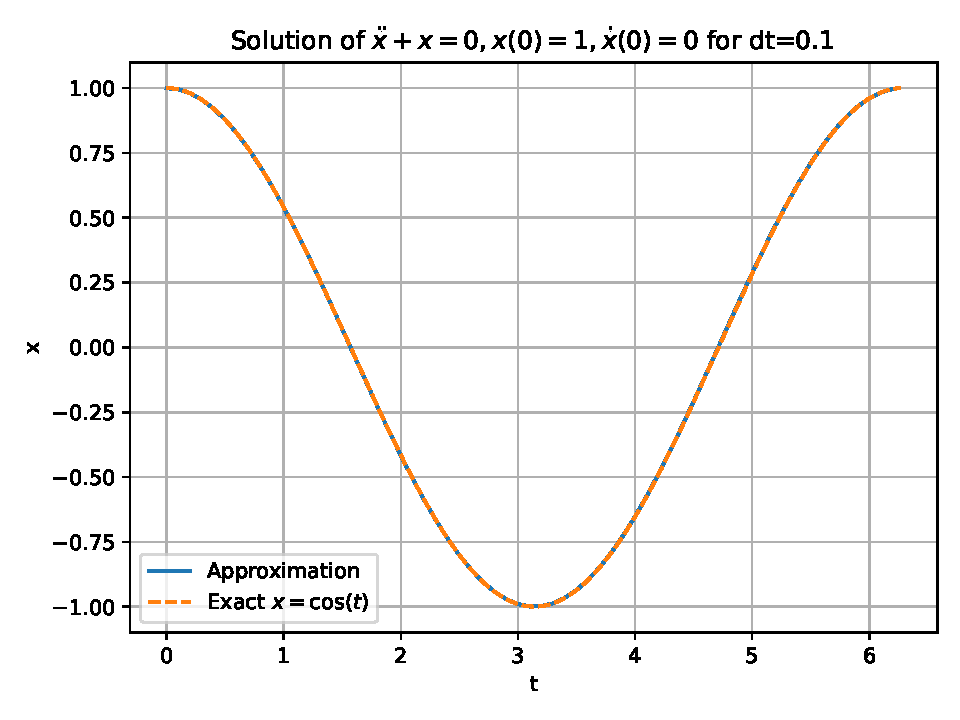
\includegraphics[width=0.8\textwidth]{figures/approx_vs_exact_dt_0_1.pdf}
  \caption{Approximate and exact solutions of the problem $\ddot{x} - x = 0, x(0)=1, \dot{x}(0)=0$ for $\Delta t = 0.1$.}
  \label{approx_vs_exact_dt_0_1}
\end{figure}


\subsection{Plotting error dependence on $t$}

Next, we want to see how absolute errors -- an absolute value of the difference between the approximate and exact solution at each $t$ -- depends on $t$. The absolute errors for $\Delta t = 1$ and $\Delta t = 0.1$ are shown on Figures \ref{abs_error_dt_1} and \ref{abs_error_dt_0_1}. We can see that globally the absolute error increases with $t$ (we ignore the periodic oscillations that make the error oscillate locally) for both time steps. We can also see that absolute errors from $\Delta t = 1$ solution are about $100$ times larger than those from $\Delta t = 0.1$ solution.

\begin{figure}[H]
  \centering
  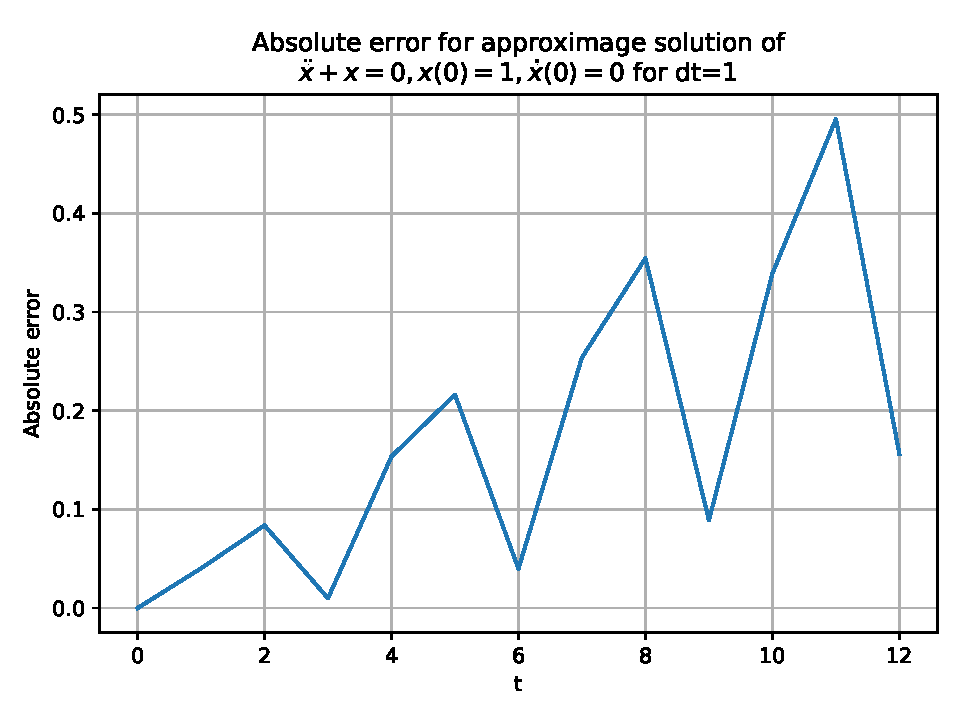
\includegraphics[width=0.8\textwidth]{figures/abs_error_dt_1.pdf}
  \caption{Absolute error of numerical solution of the problem $\ddot{x} - x = 0, x(0)=1, \dot{x}(0)=0$ for $\Delta t = 1$.}
  \label{abs_error_dt_1}
\end{figure}
\begin{figure}[H]
  \centering
  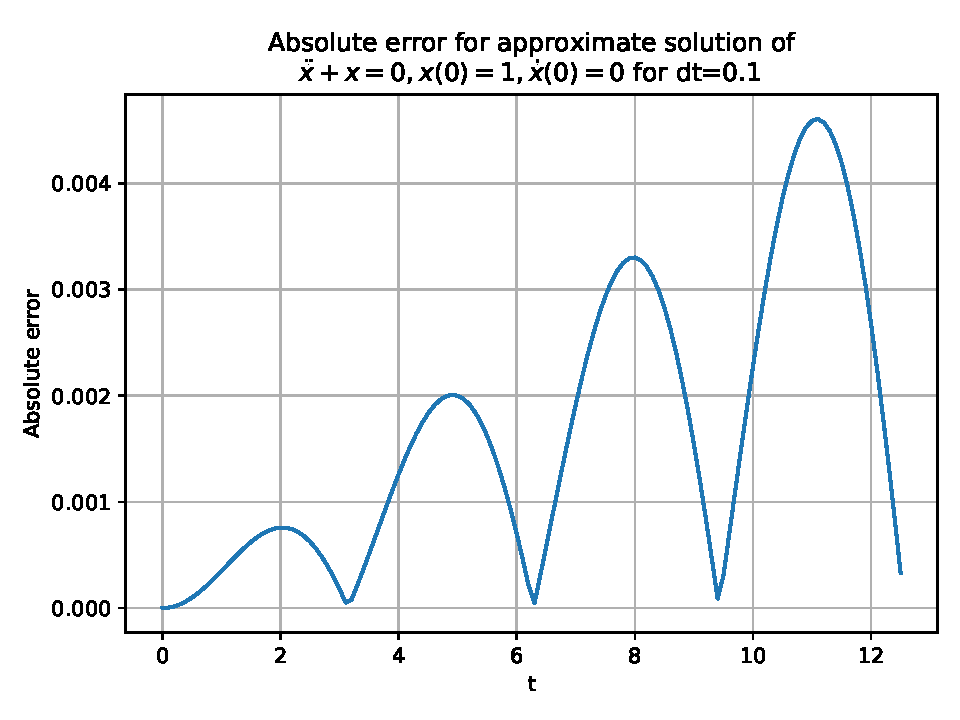
\includegraphics[width=0.8\textwidth]{figures/abs_error_dt_0_1.pdf}
  \caption{Absolute error of numerical solution of the problem $\ddot{x} - x = 0, x(0)=1, \dot{x}(0)=0$ for $\Delta t = 0.1$.}
  \label{abs_error_dt_0_1}
\end{figure}


\subsection{Dependence of errors on $\Delta t$}

Finally, we want to see how the choice of the time step affects the absolute errors. We run our Fortran program repeatedly for the following values of timesteps:
\[
  \Delta t = 1, 0.5, 0.2, 0.1, 0.05, 0.02, 0.01, 0.005, 0.002, 0.001, 0.0005.
\]
Next we calculate the absolute errors of the numerical solutions at $t=11$ on \autoref{abs_error_vs_dt}. The value $t=11$ was chosen because it corresponds to a large error on \autoref{abs_error_dt_0_1}. The log-log plot of the errors is shown on \autoref{abs_error_vs_dt}.

\begin{figure}[H]
  \centering
  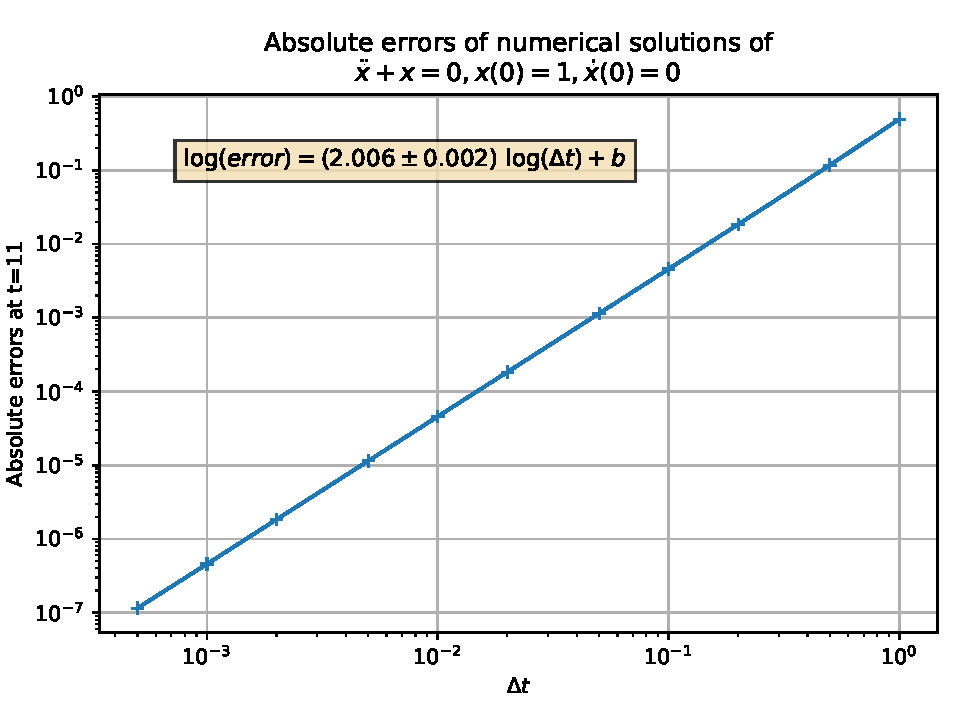
\includegraphics[width=0.8\textwidth]{figures/abs_error_vs_dt.pdf}
  \caption{Dependence of absolute errors of numerical solution of the problem $\ddot{x} - x = 0, x(0)=1, \dot{x}(0)=0$ on time step.}
  \label{abs_error_vs_dt}
\end{figure}

We can see from \autoref{abs_error_vs_dt} that there is a strong increasing linear relationship between the logarithms of the error and the time step. In order to find its slope, we calculate an equation for the line of best fit using \emph{linregress} function from the \emph{scipy} package:
\[
  \log(\textrm{error}) = (2.006 \pm 0.002) \log(\Delta t) + b,
\]
where $b$ is some value for the $y$-intercept. We can see that the slope is within three standard errors from $2$. Therefore, relation between the maximum error and the time step is, approximately:
\[
  \textrm{Global error} \sim \Delta t^2.
\]
Hence, we conclude that our numerical solution method is of the order $O(\Delta t^2)$.


\subsection{Errors for very small $\Delta t$}

We have found that errors are proportional to $\Delta t^2$. We want to see if this remains true for very small values of $\Delta t$, such as:
\[
  \Delta t = 0.0002, 0.0001, 0.00001, 0.000001, 0.0000001.
\]
The corresponding errors are shown on \autoref{abs_error_vs_dt_small_delta_t}. We can see that proportionality
\[
  \textrm{Global error} \sim \Delta t^2.
\]
no longer holds for $\Delta t < 0.0005$. Is we decrease $\Delta t$ past $\Delta t < 0.0005$, the errors start to increase, not decrease. The increasing errors could be caused by the rounding errors of the floating point numbers and arithmetic operations with those numbers. These error accumulate with each time step and may become significant for small values of $\Delta t$ and large number of time steps.

Our conjecture could be tested by modifying the Fortran program and using quadruple precision for real variables instead of the currently used double precision. If the errors for very small $\Delta t$ are indeed caused by the limitations of the floating point number system, then we expect that quadruple precision will decrease the errors for $\Delta t = 0.0002, 0.0001, 0.00001$ and maintain the proportionality
\[
  \textrm{Global error} \sim \Delta t^2.
\].
\begin{figure}[H]
  \centering
  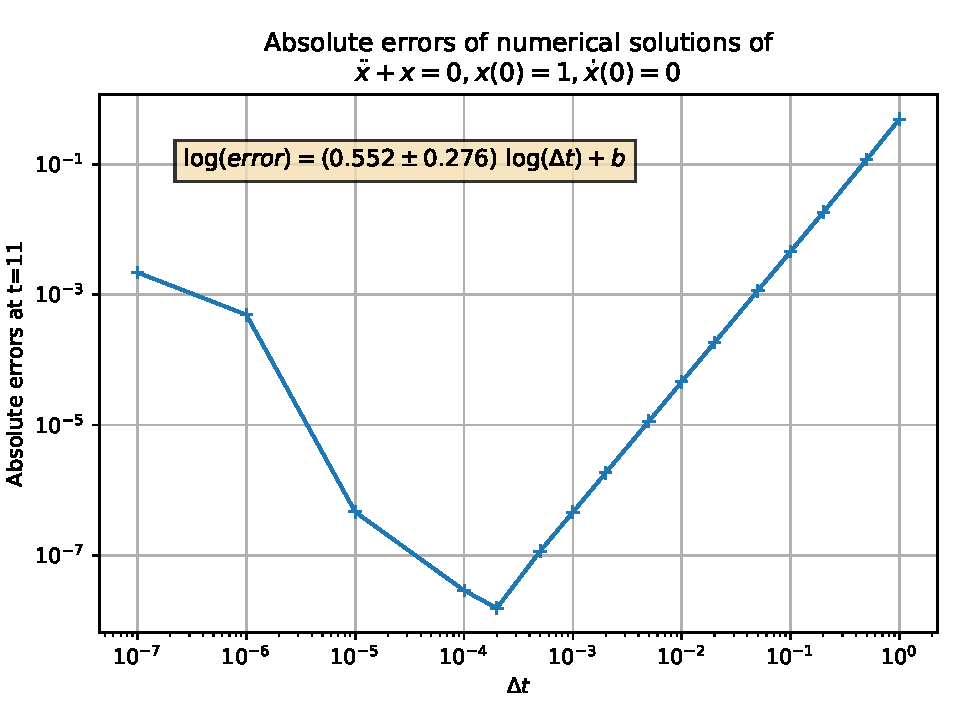
\includegraphics[width=0.8\textwidth]{figures/abs_error_vs_dt_small_delta_t.pdf}
  \caption{Dependence of absolute errors of numerical solution of the problem $\ddot{x} - x = 0, x(0)=1, \dot{x}(0)=0$ on time step including $\Delta t < 0.0005$.}
  \label{abs_error_vs_dt_small_delta_t}
\end{figure}



\subsection{Conclusion}

We wrote a Fortran program for solving the $\ddot{x} - x = 0, x(0)=1, \dot{x}(0)=0$ problem numerically. We analyzed the absolute errors of our numerical approximation of the solution. We found that global errors of our numerical method were proportional to the square of the time step when using the time steps between $0.0005$ and $1$. Time steps smaller than $0.0005$ caused the error to increase.